%Template pembuatan Tesis dengan ugmtesis.

\documentclass[tesis]{ugmtesis}

%-----------------------------------------------------------------
%Disini awal masukan untuk data tesis
%-----------------------------------------------------------------
\titleind{ANALISIS TEORETIS PEMANTULAN DAN PEMBIASAN
GELOMBANG ELEKTROMAGNETIK
PADA BAHAN MAGNETIK NON LINEAR ORDE DUA}

\titleeng{THEORETICAL ANALYSIS 
OF REFLECTION AND TRANSMISSION  
OF ELECTROMAGNETIC WAVE 
ON SECOND ORDER NONLINEAR MAGNETIC MATERIAL }

\fullname{RONIYUS MS}

\idnum{12333/I-4/0978/99}

\examdate{4 Januari 2002}

\degree{Master of Science}

\yearsubmit{2002}

\program{Ilmu Fisika}

\headprogram{Dr Jazi Eko Istiyanto}

\dept{Fisika}

\firstsupervisor{Prof. Muslim, Ph.D}

\secondsupervisor{Dr. Kamsul Abraha}

\firstexaminer{Dr. Pramudita Anggraita}

\secondexaminer{Dr. Pekik Nurwantoro, M.S}

\thirdexaminer{Dr. Agung B.S. Utomo}

%-----------------------------------------------------------------
%Disini akhir masukan untuk data tesis
%-----------------------------------------------------------------

\begin{document}

\cover

\titlepageind 

\approvalpage

\declarepage

%-----------------------------------------------------------------
%Disini awal masukan Acknowledment
%-----------------------------------------------------------------
\acknowledment
\begin{flushright}
\Large\emph\cal{Karya sederhana ini kupersembahkan \\
buat Bapak, Mama, Nenek, \\dan Adik tercinta}
\end{flushright}
%-----------------------------------------------------------------
%Disini akhir masukan untuk muka tesis
%-----------------------------------------------------------------

%-----------------------------------------------------------------
%Disini awal masukan Motto
%-----------------------------------------------------------------
\motto
\emph{Sesungguhnya dalam penciptaan langit dan bumi, dan silih bergantinya
malam dan siang terdapat tanda-tanda bagi orang-orang yang berakal, (yaitu)
orang-orang yang mengingat Allah sambil berdiri atau duduk atau dalam keadaan
berbaring dan mereka memikirkan tentang penciptaan langit dan bumi (seraya
berkata) : Ya Tuhan kami, tiadalah Engkau menciptakan ini dengan sia-sia, Maha
Suci Engkau, maka peliharalah kami dari siksa neraka.}

\begin{flushright}
(Q.S. Ali Imran : 190 - 191)
\end{flushright}

\emph{Maka apabila kamu telah selesai (dari sesuatu urusan), kerjakanlah
dengan sungguh-sungguh (urusan) yang lain.}

\begin{flushright}
(Q.S. Alam Nasyrah : 7)
\end{flushright}
%-----------------------------------------------------------------
%Disini akhir masukan untuk Motto
%-----------------------------------------------------------------

%-----------------------------------------------------------------
%Disini awal masukan untuk Prakata
%-----------------------------------------------------------------
\preface
Segala puji dan syukur semata-mata hanya untuk Allah SWT, karena atas segala
rahmat, hidayah dan bantuan-Nya jualah maka akhirnya Tesis dengan judul
Analisis Teoretis Pemantulan dan Pembiasan Gelombang Elektromagnet Pada
Bahan Magnetik Non Linear Orde Dua ini telah selesai penulis susun.

Telah banyak bantuan yang penulis peroleh selama dalam penulisan Tesis ini
, untuk itu tak lupa penulis ucapkan terima kasih yang sebesar-besarnya
kepada:
\begin{enumerate}
\item{Bapak dan Mama yang selama ini telah sabar membimbing dan mendoakan
penulis tanpa kenal untuk selama-lamanya,}
\item{Prof. Drs. H. Muslim, Ph. D, selaku Pembimbing Utama, yang telah
memberikan ilmunya kepada penulis serta dengan penuh kesabaran membimbing penulis,}
\item{Drs. Kamsul Abraha, Ph. D, selaku Pembimbing Pendamping yang telah
memberikan inspirasi kepada penulis,} 
\item{Dr. Pekik Nurwantoro dan Dr. rer. nat. M. Farchani Rasyid
yang telah memperkenalkan sistem operasi LINUX dan \LaTeX{} kepada penulis serta
memberikan bimbingan penggunaan \LaTeX{} tersebut dengan sabar,} 
\item{Segenap staf dan karyawan di jurusan Fisika FMIPA UGM, yang telah
banyak bekerjasama dengan penulis selama belajar di FMIPA UGM,} 
\item{Sahabat saya M. Rizal Ginanjar, yang selalu bersedia membantu penulis ketika
menyelesaikan masalah-masalah komputer.} 
\end{enumerate}

Tesis ini tentunya tidak lepas dari segala kekurangan dan kelemahan, untuk itu
segala kritikan dan saran yang bersifat membangun guna kesempurnaan Tesis ini
sangat diharapkan. Semoga tesis ini dapat bermanfaat bagi kita semua dan lebih
khusus lagi bagi pengembagan ilmu fisika.

\begin{tabular}{p{7.5cm}c}
&Yogyakarta, 12 Mei 1994\\
&\\
&\\
&Penulis
\end{tabular}
%-----------------------------------------------------------------
%Disini akhir masukan Prakata
%-----------------------------------------------------------------

\tableofcontents
\listoftables
\listoffigures
%\lambang

%-----------------------------------------------------------------
%Disini awal masukan Intisari
%-----------------------------------------------------------------
\begin{abstractind}
Telah dilakukan telaah teoretis mengenai proses pemantulan dan pembiasan
gelombang elektromagnet dalam tinjauan klasik, termasuk pembahasan tentang
pembangkitan frekuensi harmonik kedua pada bahan magnetik
\emph{semi-infinite}. Telaah ini sebagai kelanjutan dari telaah sebelumnya
tentang perambatan gelombang elektromagnet yang terjadi karena respon non
linear di dalam sebuah bahan magnetik \emph{infinite}. Gelombang
elektromagnet harmonic kedua (SHEM) yang terpantul dan terbias ini sangat
dipengaruhi oleh gelombang elektromagnet harmonik pertama yang terpantul dan
terbias yang dibangkitkan oleh gelombang datang. Prosentase dari
pemantulan dan pembiasan gelombang SHEM ini lebih kecil daripada gelombang
harmonik pertama. Dari telaah teoretis ini juga didapatkan informasi dari 
bahan $\mathrm{FeF_2}$ yang merupakan salah satu dari jenis bahan
antiferromagnet uniaksial, bahwa perbandingan antara
$\frac{R^{(2)}}{T^{(2)}_1}$ dan $\frac{T^{(2)}_2}{T^{(2)}_1}$ dengan
$R^{(2)}$, $T^{(2)}_1$ dan $T^{(2)}_2$ berturut-turut adalah reflektansi
gelombang SHEM, transmitansi gelombang SHEM yang terbias pertama dan
transmitansi gelombang SHEM yang terbias kedua, memiliki
sifat resiprokal terhadap perubahan tanda $H_0$ (medan magnet konstan dari
luar) atau perubahan tanda $\phi$ (sudut gelombang datang terhadap garis
normal), tetapi sifat-sifat ini tidak dijumpai pada konfigurasi Faraday
polarisasi p. Diharapkan telaah ini dapat dilanjutkan pada penelitian
berikutnya yang mengarah pada pemanfaatan lebih lanjut gejala non linear dalam
bahan magnetik tersebut. 

\bigskip
Kata-kata kunci : bahan magnet, non linear orde dua, optika.
\end{abstractind}
%-----------------------------------------------------------------
%Disini akhir masukan Intisari
%-----------------------------------------------------------------

%-----------------------------------------------------------------
%Disini awal masukan untuk Abstract
%-----------------------------------------------------------------
\begin{abstracteng}
A theoretical investigation of classical electromagnetic wave reflection and
transmission process involving second harmonic frequency generation by a
semi-infinite magnetic material has been carried out. This investigation is
the continuation of a previous investigation on nonlinear propagation of
electromagnetic wave inside an infinite magnetic medium. The reflected and
transmitted of second harmonic electromagnetic (SHEM) wave is strongly
influenced by reflected and transmitted of first harmonic electromagnetic wave
generated by the incoming wave. The percentage of the reflected and
transmitted of the SHEM wave is much smaller than those of the first
harmonics. From the theoretical analysis it is found that the for uniaxial
antiferromagnet materials such as $\mathrm{FeF_2}$, the ratio
$\frac{R^{(2)}}{T^{(2)}_1}$ and $\frac{T^{(2)}_2}{T^{(2)}_1}$ where $R^{(2)}$,
$T^{(2)}_1$ and $T^{(2)}_2$ are reflectance of the SHEM wave, first wave
transmittance of SHEM wave and second wave transmittance of SHEM wave,
succesfully, have resiprocal properties when the sign of $H_0$ (constant
external magnetic field) or $\phi$ (angle of incidence wave) is changing.
This does not occur in Faraday's configuration p polarization. It is
expected that this investigation can be extended into a further
investigation involving applications of nonlinear effects in magnetic
materials. 

\bigskip
Keywords : magnetic material, second order nonlinear, optics.
\end{abstracteng}
%-----------------------------------------------------------------
%Disini akhir masukan Abstract
%-----------------------------------------------------------------

%-----------------------------------------------------------------
%Disini awal masukan untuk Bab
%-----------------------------------------------------------------
\chapter{PENDAHULUAN}
\section{Latar Belakang Masalah}
Dewasa ini, telaah optika linear maupun non linear orde dua pada bahan listrik
dan dalam tinjauan medan listriknya telah dilakukan secara lengkap. Telaah
tersebut melingkupi telaah klasik dan kuantum mengenai kerentanan listrik non
linear orde dua \citep{ar}, perhitungan intensitas gelombang elektromagnet
berfrekuensi sudut $2\omega$ yang dihasilkan oleh sebuah bahan dielektrik
non li\-near orde dua yang dikenai gelombang elektromagnet dari luar \citep{ar},
tinjauan teoretis tentang gejala pemantulan dan pembiasan gelombang
elektromagnet berfrekuensi sudut $2\omega$ \citep{blpr}, hukum-hukum kekekalan
yang menyertai gejala optika non linear orde dua \citep{bl}, percobaan
pengukuran intensitas gelombang elektromagnet berfrekuensi sudut $2\omega$
\citep{ar}, percobaan pembiasan optika non linear \citep{ma} dan penggunaan bahan
dielektrik non linear untuk memproses informasi secara digital dengan kelajuan
tinggi \citep{cot}.  

Sejauh pengetahuan penulis, telaah serupa belum begitu lengkap dilakukan pada
bahan magnetik dan dalam tinjauan medan magnetiknya. Hingga kini telaah yang
telah dilakukan antara lain adalah telaah klasik mengenai kerentanan magnetik
linear dalam bahan magnetik yang terdiri dari dua sub-kisi dengan sumbu mudah
kemagnetannya memiliki sudut sebarang terhadap medan magnet konstan dari luar
$\overrightarrow{H}_0$ \citep{ab4}. Yang dimaksud dengan sub-kisi adalah
bentuk susunan atom-atom dalam sebuah kisi yang dapat dikelompokkan menjadi
beberapa kelompok kecil, sedangkan sumbu mudah (\emph{easy axis}) adalah arah
yang disukai oleh magnetisasi kristal. Telaah lain yang dilakukan adalah
mengenai kerentanan magnetik non linear orde dua yang terdiri dari dua
sub-kisi dengan sumbu mudahnya tegak lurus pada medan magnet konstan dari luar
$\overrightarrow{H}_0$ \citep{mar}.

Keistimewaan bahan yang terdiri dari dua sub-kisi ini adalah karena bahan
magnet jenis seperti ini sudah terbukti secara eksperimental dapat memberikan
respon optika linear sehingga diharapkan bahan jenis ini pun dapat memberikan
respon optika non linear orde dua \citep{ab4}. Contoh bahan magnetik yang telah
diselidiki respon linearnya adalah antiferromagnet uniaksial FeF$_2$
\citep{ab4}. Telaah lain yang telah dilakukan adalah perhitungan intensitas
gelombang elektromagnet (dalam tinjauan medan magnetnya) berfrekuensi sudut
$2\omega$ pada bahan magnetik non linear orde dua \citep{mar}. Kemudian, telah
pula ditelaah percobaan pemantulan dan pembiasan pada bahan magnetik dengan
menggunakan konfigurasi Voigt dan Faraday \citep{ab5}. Konfigurasi Voigt adalah
konfigurasi dengan suatu medan magnet konstan homogen dari luar
$\overrightarrow{H}_0$ dipasang tegak lurus terhadap bidang datang
(\emph{plane of incidence}) yang berbeda dari konfigurasi Faraday, yaitu suatu
konfigurasi dengan medan magnet luar $\overrightarrow{H}_0$ yang konstan dan
homogen dipasang sejajar terhadap bidang datang. Selain itu juga telah
dilakukan telaah teoretis rotasi optika non linear pada bahan magnetik
semikonduktor Cd$_0.75$Mn$_0.25$Te dengan menggunakan tinjauan medan
listrik \citep{bor}.

Optika merupakan suatu gejala interaksi antara gelombang elektromagnet yang
terdiri dari gelombang listrik dan gelombang magnet yang saling terkait
deng\-an bahan yang dilewatinya dimana panjang gelombang elektromagnet
tersebut terbentang dari 10$^{-16}$ m sampai dengan 10$^{8}$ m \citep{hal}.
Jadi gelombang elektromagnet tersebut tidak hanya mencakup gelombang
elektromagnet dengan frekuensi berada pada daerah spektrum cahaya tampak
(seperti yang dikenal dalam kehidupan sehari-hari dengan $\lambda$-nya dari 10
nm sampai dengan 0,1 mm), tetapi juga gelombang elektromagnet yang
berada di sekitarnya yang tidak termasuk cahaya tampak, misalnya sinar
infra merah dan ultra ungu. Bahan yang ada di alam juga dapat berupa bahan
yang lebih bersifat listrik atau lebih bersifat magnet. Menurut persamaan
Maxwell, gelombang elektromagnet terdiri dari gelombang listrik dan
gelombang magnet yang saling terkait, jadi tidak pernah dijumpai adanya
gelombang listrik yang dapat berdiri sendiri dan begitu pula halnya pada
gelombang magnet. Jika suatu gelombang elektromagnet mengenai bahan listrik,
maka gelombang listriknya akan berpengaruh lebih besar dalam menginduksi bahan
tersebut, sehingga energi gelombang listriknya akan berkurang dari semula
karena telah mengalami suatu proses induksi di dalam bahan, demikian pula
halnya jika gelombang elektromagnet mengenai bahan maka gelombang magnetnya
akan lebih berperan daripada gelombang listriknya.

Dengan demikian telaah yang lengkap secara teoretis maupun secara
eks\-pe\-ri\-men dalam bidang optika magnetik sangat diperlukan, seperti yang
telah dilakukan selama ini pada bahan listrik. Hal ini diperlukan agar telaah
sifat optik bahan secara fisis menjadi lengkap, yaitu mencakup tinjauan
listrik maupun magnetnya.

 \nomenclature{$\delta$}{Lambang delta}%

\section{Perumusan Masalah}
Dari latar belakang di atas, maka dapat dirumuskan beberapa masalah yang
"\emph{up to date}" untuk penulisan tesis ini. Masalah-masalah tersebut berada
dalam ruang lingkup gejala optika non linear orde dua sebagai kelanjutan yang
telah dilakukan sebelumnya oleh penulis pada bahan magnetik \citep{mar},
sedangkan sistem satuan yang digunakan dalam penelitian ini adalah Sistem
Internasional (SI). Secara terperinci masalah-masalah yang dimaksud mencakup
hal-hal sebagai berikut:

\begin{enumerate}
\item Sebelum membahas gejala pemantulan dan pembiasan gelombang
elektromagnet berfrekuensi sudut $2\omega$ pada bahan magnetik non linear
orde dua sebagai topik utama, terlebih dahulu akan dibahas gejala pemutaran
arah polarisasi gelombang elektromagnet di dalam bahan magnet linear maupun non
linear orde dua, isotrop maupun anisotrop dengan telaah dilakukan pada komponen
magnetiknya; dan

\item Gejala pemantulan dan pembiasan gelombang elektromagnet berfrekuensi sudut
$2\omega$ pada bahan magnetik yang bergeometri \emph{semi-infinite} yang
diberi atau tanpa tambahan $\overrightarrow{H}_0$.  Penggunaan bahan
bergeometri \emph{semi-infinite} dikarenakan penelitian ini hanya membahas
perilaku gelombang elektromagnet di bidang batas.    
\end{enumerate}

\section{Tujuan Penelitian}
Berdasarkan masalah-masalah di atas maka cakupan tujuan penelitian ini secara
rinci dapat dirumuskan sebagai berikut:
\begin{enumerate}

\item Telaah mengenai pemutaran arah polarisasi gelombang elektromagnet pada
bahan magnetik bertujuan untuk mendapatkan gambaran yang jelas men\-gena\-i
perilaku gelombang elektromagnet dalam bahan magnet; dan

\item Telaah mengenai gejala pemantulan dan pembiasan gelombang elektromagnet
berfrekuensi sudut $2\omega$ oleh permukaan bahan magnetik non linear orde dua 
bertujuan untuk menghitung reflektansi serta transmitansi permukaan bahan
magnet tersebut dengan atau tanpa medan magnet tambahan
$\overrightarrow{H}_0$ yang statis dan homogen. 
\end{enumerate}

\section{Manfaat Penelitian}
Dengan mengacu pada tujuan penelitian di atas, maka manfaat penelitian
meliputi hal-hal sebagai berikut:

\begin{enumerate}
\item Telaah ini dapat menjadi salah satu acuan dalam merumuskan proses
pemantulan dan pembiasan gelombang elektromagnet berfrekuensi sudut $2\omega$
pada bahan magnetik non linear orde dua yang bergeometri \emph{semi-infinite};
dan

\item Selain itu telaah ini juga dapat menjadi salah satu acuan teoretik dalam
merancang percobaan mengenai pemantulan dan pembiasan gelombang elektromagnet
berfrekuensi sudut $2\omega$ pada bahan magnetik non linear orde dua.

\end{enumerate}

\section{Keaslian Tesis}
Berdasarkan pelacakan literatur dan internet yang ada ternyata permasalahan
yang dikaji dalam tesis ini belum pernah diteliti.

\chapter{DASAR TEORI}                
Sebelum memasuki perhitungan yang lebih jauh, perlu diketahui bahwa di dalam
tesis ini digunakan kesepakatan Einstein yang memungkinkan peniadaan penulisan
lambang $\Sigma$ secara eksplisit apabila terdapat indeks yang muncul berulang
dua kali, jadi munculnya indeks berulang tersebut selalu berarti adanya
perintah penjumlahan terhadap bentuk yang memuatnya meliputi
seluruh jangkauan indeks kecuali kalau dinyatakan lain, misalnya indeksnya
ditulis sebagai (a) (dengan kurung).

\section{Ungkapan Gelombang Magnet Di Dalam Bahan Magnet}
Persamaan-persamaan Maxwell dalam satuan SI untuk bahan, tanpa rapat muatan dan
rapat arus listrik dengan tetapan permitivitas ($\epsilon$) mutlak berbentuk
skalar \cite{wangs} adalah 
\begin{displaymath}
\textrm{(a) }
\nabla\cdot\overrightarrow{D}(\vec r,t)=0;\quad\quad 
\textrm{(c) }
\nabla\cdot\overrightarrow{B}(\vec r,t)=0;
\end{displaymath}
\begin{equation}
\label{2.1}
\textrm{(b) }
\nabla\times\overrightarrow{E}(\vec
r,t)=-\frac{\partial\overrightarrow{B}(\vec r,t)}{\partial{t}},\quad\quad
\textrm{(d) }
\nabla\times\overrightarrow{H}(\vec
r,t)=\frac{\partial\overrightarrow{D}(\vec r,t)}{\partial t}
\end{equation} dan
\begin{equation}
\label{2.2}
\textrm{(a) }\overrightarrow{D}(\vec r,t)=\epsilon\overrightarrow{E}(\vec
r,t),\qquad
\textrm{(b) }\overrightarrow{B}(\vec r,t)=\mu_0\Big(
(\overrightarrow{H}(\vec r,t)+\overrightarrow{M}(\vec r,t) \Big).
\end{equation} Disini $\mu_0=4\pi\cdot{10}^{-7}$ H/m adalah permeabilitas
mutlak ruang hampa.
\subsection{Bahan Magnet Isotrop Linear}
Magnetisasi linear untuk bahan magnet dengan parameter kerentanan
magnetik linear $\chi^{(1)}$ berbentuk 
\begin{equation}
\label{2.3}
\overrightarrow{M}^{(\mathrm{L})}(\vec
r,t)=\overrightarrow\chi^{(1)}\overrightarrow{H}(\vec r,t).
\end{equation} Jika observabel gelombang magnetnya merambat sebagai
gelombang datar harmonik berfrekuensi sudut $\omega$, vektor gelombangnya
adalah $\vec k$, serta dalam penyajian kompleks, maka
\begin{equation} 
\label{2.4}
\overrightarrow{M}^{(\mathrm{L})}(\vec
r,t)=\overrightarrow{M}^{(\mathrm{L})}_0(\vec r,t)\exp\Big[ i(\vec
k\cdot\vec r-\omega{t}) \Big]
\end{equation}dan
\begin{equation}
\label{2.5}
\overrightarrow{H}(\vec r,t)=\overrightarrow{H}_0(\vec r,t)\exp\Big[ i(\vec
k\cdot\vec r-\omega{t}) \Big].
\end{equation} Substitusi pers.(\ref{2.4}) dan pers.(\ref{2.5}) ke
pers.(\ref{2.3}) menghasilkan
\begin{equation}
\label{2.6}
{M}^{(\mathrm{L})}_\mathrm{0i}=\chi^{(1)}_\mathrm{ij}H_{\mathrm{0j}};\textrm{i
= x, y dan z}. 
\end{equation} Untuk bahan magnet isotrop linear,
$\chi^{(1)}_\mathrm{ij}=0$ kecuali
\begin{equation}
\label{2.7}
\chi^{(1)}_\mathrm{xx}=\chi^{(1)}_\mathrm{yy}=\chi^{(1)}_\mathrm{zz}=\chi^{(1)},
\end{equation} sehingga pers.(\ref{2.3}) dapat dituliskan kembali menjadi
\begin{equation}
\label{2.8}
\overrightarrow{M}^{(\mathrm{L})}(\vec
r,t)=\chi^{(1)}\overrightarrow{H}(\vec r,t). 
\end{equation} Substitusi pers.(\ref{2.3}) ke pers.(\ref{2.2}.b) menghasilkan
bentuk
\begin{equation}
\label{2.9}
\overrightarrow{B}(\vec r,t)=\mu\overrightarrow{H}(\vec r,t),
\end{equation}dengan permeabilitas mutlak
\begin{equation}
\label{2.10}
\mu=\mu_0\mu_{\mathrm{r}},
\end{equation} $\mu_{\mathrm{r}}$ adalah permeabilitas relatif bahan yang berbentuk
\begin{equation}
\label{2.11}
\mu_{\mathrm{r}}=1+\chi^{\mathrm{(1)}}.
\end{equation}

Substitusi pers.(\ref{2.2}.a) dan
pers.(\ref{2.9}) ke pers.(\ref{2.1}) memberikan persamaan Maxwell untuk
gelombang elektromagnet yang merambat dalam bahan magnet yang linear dan
isotrop, yaitu
\begin{displaymath}
\textrm{(a) }
\nabla\cdot\overrightarrow{E}(\vec r,t)=0;\quad\quad
\textrm{(c) }
\nabla\cdot\overrightarrow{H}(\vec r,t)=0;
\end{displaymath}
\begin{equation}
\label{2.12}
\textrm{(b) }
\nabla\times\overrightarrow{E}(\vec
r,t)=-\mu\frac{\partial\overrightarrow{H}(\vec r,t)}{\partial{t}};\quad\quad
\textrm{(d) }
\nabla\times\overrightarrow{H}(\vec
r,t)=\epsilon\frac{\partial\overrightarrow{E}(\vec r,t)}{\partial{t}}.
\end{equation}

Dari pers.(\ref{2.12}.a) diperoleh informasi bahwa vektor amplitudo
gelombang listrik $\overrightarrow{E}(\vec r,t)$ yang merambat dalam
medium isotrop akan tegak lurus terhadap arah perambatan gelombang
$\overrightarrow{k}$. Misalkan untuk perambatan ke arah sumbu z, maka bentuk
gelombang listrik dengan pengutupan vektor amplitudonya ke arah
$\hat{u}$ berbentuk
\begin{equation}
\label{2.13}
\overrightarrow{E}(\vec r,t)=E_0\exp\Big[ i(kz-\omega t) \Big]\hat{u},
\end{equation} agar bentuk ini memenuhi pers.(\ref{2.12}.a), maka
harus dipenuhi $\hat{u}\cdot\hat{z}=0$, sehingga dapat diambil
$\hat{u}=\hat{x}$. Demikian pula untuk gelombang $\overrightarrow{H}(\vec
r,t)$ nya berbentuk
\begin{equation}
\label{2.14}
\overrightarrow{H}(\vec r,t)=H_0\exp\Big[ i(kz-\omega t)
\Big]\hat{u_\mathrm{H}}, 
\end{equation}
agar bentuk ini memenuhi pers.(\ref{2.12}.c), maka harus dipenuhi
$\hat{u_\mathrm{H}}\cdot\hat{z}=0$. Selanjutnya menurut pers.(\ref{2.12}.b)
\begin{equation} 
\label{2.15} 
ikE_0\exp\Big[ i(kz-\omega t)
\Big]\hat{y}=-\mu(-i\omega)H_0\exp\Big[ i(kz-\omega t) \Big]\hat{u_\mathrm{H}}
\end{equation} Jadi diperoleh $\hat{u_\mathrm{H}}=\hat{y}$ yang dapat memenuhi 
$\hat{u_\mathrm{H}}\cdot\hat{z}=\hat{y}\cdot\hat{z}=0$.
Selain itu dari pers.(\ref{2.15}) didapatkan pula  
\begin{equation}
\label{2.16}
H_0=\frac{k}{\mu\omega}E_0,
\end{equation} sehingga jika digambarkan akan tampak seperti pada
Gb.\ref{gb2.1}, dengan $\overrightarrow{S}(\vec r,t)$ pada Gb.\ref{gb2.1}
adalah vektor Poynting sesaat \citep{wangs} yang nilainya ditentukan oleh
\begin{equation}
\label{2.17}
\overrightarrow{S}(\vec r,t)=\overrightarrow{E}(\vec
r,t)\times\overrightarrow{H}(\vec r,t).  
\end{equation}

\begin{figure}[ht]
\begin{center}
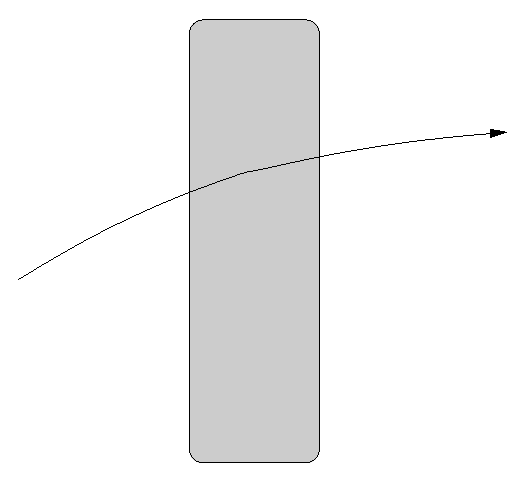
\includegraphics[height=45mm,width=70mm]{gb21}
\caption{Perambatan gelombang elektromagnet di dalam bahan magnet
isotrop linear}
\label{gb2.1}
\end{center}
\end{figure} 

Pembuktian lain adalah dengan menggunakan pers.(\ref{2.12}.b) yang dapat
di\-tu\-lis\-kan kembali menjadi
\begin{equation}
\label{2.18}
\overrightarrow{H}(\vec r,t)=\frac{1}{\mu\omega}\vec k
\times\overrightarrow{E}(\vec r,t).
\end{equation} Demikian pula pers.(\ref{2.12}.d) dapat dituliskan
kembali sebagai 
\begin{equation}
\label{2.19}
\overrightarrow{E}(\vec r, t)=-\frac{1}{\omega\epsilon} \vec
k\times\overrightarrow{H}(\vec r, t).
\end{equation}
%-----------------------------------------------------------------
%Disini akhir masukan Bab
%-----------------------------------------------------------------

%-----------------------------------------------------------------
%Disini awal masukan untuk Daftar Pustaka
%-----------------------------------------------------------------
\begin{thebibliography}{99}
\bibitem[Abraha(1995)]{ab5}
Abraha, K., 1995, Ph. D. Thesis: \emph{Theory of Surface
Polaritons and Far Infrared Reflectivity of Antiferromagnets, Rare Earth
Metals and Ferrimagnets}, University of Essex, England, hal.35 - 79 dan 236 -
254.  

\bibitem[Abraha \emph{dkk}(1994)]{ab4}
Abraha, K., Brow, T. E., Dumelow, T., Parker, T. J. dan Tilley, D. R.,  1994,
Oblique-incidence Far Infrared Reflectivity Study Of The Uniaxial
antiferromagnet FeF$_2$, \emph{Physical Review B}, Vol.50, No.10 September
1994, hal.6808 - 6816. 

\bibitem[Arkundato(1995)]{ar}
Arkundato, A.,  1995, Skripsi S1: \emph{Aspek Klasik dan Kuantum Optika Non
Linear}, Jurusan Fisika FMIPA UGM Yogyakarta Indonesia, hal.2, 9 - 14, 58 - 60
dan 146.

\bibitem[Bloembergen dan Pershan(1962)]{blpr}
Bloembergen, N. dan Pershan, P. S., 1962, Light Waves at The
Boundary of Nonlinear Media, \emph{Physical Review}, Vol.128, Number 2,
hal.606 - 622. 

\bibitem[Bloembergen(1980)]{bl}
Bloembergen, N., 1980, Conservation laws in nonlinear
optics, \emph{Journal of Optical Society of America}, Vil.70, No.12 Desember
1980, hal.1429 - 1436.

\bibitem[Budker \emph{dkk}(1999)]{bud}
Budker, D., Orlando, D. J. dan Yaschuk, V., 1999,
Nonlinear laser spectroscopy and magnet-optics, \emph{American
Journal Physics}, Vol.67, No.7 July 1999, hal.584 - 592.

\bibitem[Cotter \emph{dkk}(1999)]{cot}
Cotter, D., Maning, R. J., Blow, K. J., Ellis, A. D., Kelly, A. E.,
Nesset, D., Phillips, I. D., Poustie A. J. dan Rogers, D. C., 1999,
Nonlinear Optics for High-Speed Digital Information Processing,
\emph{SCIENCE}, Vol.286, 19 November 1999, hal.1523 - 1528.

\bibitem[Halliday dan Resnick(1986)]{hal}
Halliday, D. dan Resnick, R., 1986, \emph{Fisika Edisi Ke-3
Jilid 2}, diterjemahkan oleh Silaban, P. dan Sucipto, E., Penerbit Erlangga,
hal.537 - 568. 

\bibitem[Jackson(1999)]{jack}
Jackson, J. D., 1999, \emph{Classical Electrodynamics}, John
Wiley and Sons, New York, USA, hal.278 - 282.

\bibitem[Marjunus(1999)]{mar}
Marjunus, R., 1999, Skripsi S1: \emph{Analisis Teoretis Optika
Non Linear Dalam Bahan Megnetik}, Jurusan Fisika FMIPA UGM Yogyakarta
Indonesia, hal.1 - 76.

\bibitem[Matlin \emph{dkk}(1997)]{ma}
Matlin, M. D. dan McGee, D. J., 1997, Photorefractive nonlinear
optics in the undergraduate physics laboratory, \emph{American Journal
Physics}, Vol.65, No.7 July 1997, hal.622 - 634.

\bibitem[Wangsness(1979)]{wangs}
Wangsness, R. K., 1979, \emph{Electromagnetic Fields}, John
Wiley and Sons, New York, USA, hal.457 - 475.
\end{thebibliography}
%-----------------------------------------------------------------
%Disini akhir masukan Daftar Pustaka
%-----------------------------------------------------------------

%-----------------------------------------------------------------
%Disini awal masukan untuk Lampiran
%-----------------------------------------------------------------
\appendix
\chapter{UNGKAPAN GELOMBANG MAGNET DI DALAM BAHAN MAGNET NON LINEAR ORDE
DUA} 

Pembahasan pada lampiran ini dimulai dari bentuk gelombang magnet di dalam
bahan magnet anisotrop non linear orde dua seperti yang tercantum pada
pers.(\ref{2.19}) yaitu 
\begin{displaymath}
\overrightarrow{H}(\vec r,t)=\frac{1}{2}\bigg\{
\overrightarrow{H}^\mathrm{(1)}_0\exp\Big[ i(\vec
k^\mathrm{(1)}\cdot\vec r -\omega{t})
\Big]+\overrightarrow{H}^\mathrm{(2)}_0\exp\Big[ i(\vec
k^\mathrm{(2)}\cdot\vec r -2\omega{t}) \Big] + cc \bigg\},
\end{displaymath} sehingga diperoleh bentuk berikut ini
\begin{displaymath}
H_\mathrm{0j}(\vec r,t)H_\mathrm{0k}(\vec r,t)=\frac{1}{4}\bigg\{H^\mathrm{(1)}_\mathrm{0j}H^\mathrm{(1)}_\mathrm{0k}\exp\Big[ i(2\vec
k^\mathrm{(1)}\cdot\vec r -2\omega{t})
\Big]+2H^\mathrm{(1)}_\mathrm{0j}H^\mathrm{(1)\ast}_\mathrm{0k}
\end{displaymath} \begin{displaymath}
+2H^\mathrm{(1)}_\mathrm{0j}H^\mathrm{(2)}_\mathrm{0k}\exp\Big[ i((\vec
k^\mathrm{(1)}+\vec k^\mathrm{(2)})\cdot\vec r -3\omega{t}) \Big]
+2H^\mathrm{(1)}_\mathrm{0j}H^\mathrm{(2)\ast}_\mathrm{0k}\exp\Big[ i((\vec
k^\mathrm{(1)}-\vec k^\mathrm{(2)})\cdot\vec r +\omega{t}) \Big]
\end{displaymath}
\begin{displaymath}
+H^\mathrm{(1)\ast}_\mathrm{0j}H^\mathrm{(1)\ast}_\mathrm{0k}\exp\Big[
-i(2\vec k^\mathrm{(1)}\cdot\vec r-2\omega{t}) \Big]
+2H^\mathrm{(1)\ast}_\mathrm{0j}H^\mathrm{(2)}_\mathrm{0k}\exp\Big[-i((\vec
k^\mathrm{(1)}-\vec k^\mathrm{(2)})\cdot\vec r +\omega{t}) \Big]
\end{displaymath}
\begin{displaymath}
+2H^\mathrm{(1)\ast}_\mathrm{0j}H^\mathrm{(2)\ast}_\mathrm{0k}\exp\Big[-i((\vec
k^\mathrm{(1)}+\vec k^\mathrm{(2)})\cdot\vec r -3\omega{t}) \Big]
+H^\mathrm{(2)}_\mathrm{0j}H^\mathrm{(2)}_\mathrm{0k}\exp\Big[i(2\vec
k^\mathrm{(2)}\cdot\vec r -4\omega{t}) \Big]
\end{displaymath}
\begin{equation}
\label{4.1}
+2H^\mathrm{(2)}_\mathrm{0j}H^\mathrm{(2)\ast}_\mathrm{0k}
+H^\mathrm{(2)\ast}_\mathrm{0j}H^\mathrm{(2)\ast}_\mathrm{0k}\exp\Big[-i(2\vec
k^\mathrm{(2)}\cdot\vec r -4\omega{t}) \Big] \bigg\},
\end{equation} yang mengakibatkan magnetisasi di dalam bahan berbentuk
\begin{equation} 
\label{4.2}
M_\mathrm{i}=M^\mathrm{(L)}_\mathrm{i}+M^\mathrm{(NL)}_\mathrm{i},
\end{equation} dengan
\begin{displaymath}
M^\mathrm{(L)}_\mathrm{i}=\frac{1}{2}\bigg\{
\chi^\mathrm{(1)}_\mathrm{ij}(\omega)H^\mathrm{(1)}_\mathrm{0j}\exp\Big[ i(\vec
k^\mathrm{(1)}\cdot\vec r-\omega{t}) \Big]
+\chi^\mathrm{(1)}_\mathrm{ij}(2\omega)H^\mathrm{(2)}_\mathrm{0j}\exp\Big[
i(\vec k^\mathrm{(2)}\cdot\vec r-2\omega{t}) \Big]
\end{displaymath}
\begin{equation}
\label{4.3}
+\chi^\mathrm{(1)}_\mathrm{ij}(\omega)H^\mathrm{(1)\ast}_\mathrm{0j}\exp\Big[ -i(\vec k^\mathrm{(1)}\cdot\vec r
-\omega{t}) \Big]
+\chi^\mathrm{(1)}_\mathrm{ij}(2\omega)H^\mathrm{(2)\ast}_\mathrm{0j}\exp\Big[ -i(\vec k^\mathrm{(2)}\cdot\vec r -2\omega{t}) \Big] \bigg\}
\end{equation}

\begin{equation}
\label{4.4}
M^\mathrm{(NL)}_\mathrm{i}=\chi^\mathrm{(2)}_\mathrm{ijk}
H_\mathrm{0j}(\vec r,t)H_\mathrm{0k}(\vec r,t).
\end{equation}
Selain itu dalam koordinat Cartesan
\begin{displaymath}
\nabla^2H_\mathrm{i}=-\frac{1}{2}\bigg\{
(k^\mathrm{(1)})^2H^\mathrm{(1)}_\mathrm{0i}\exp\Big[ i(\vec
k^\mathrm{(1)}\cdot\vec r -\omega{t})
\Big]
+(k^\mathrm{(2)})^2H^\mathrm{(2)}_\mathrm{0i}\exp\Big[ i(\vec
k^\mathrm{(2)}\cdot\vec r -2\omega{t}) \Big]
\end{displaymath}
\begin{equation}
\label{4.5}
+(k^\mathrm{(1)})^2H^\mathrm{(1)\ast}_\mathrm{0i}\exp\Big[ i(\vec
k^\mathrm{(1)}\cdot\vec r -\omega{t}) \Big]
+(k^\mathrm{(2)})^2H^\mathrm{(2)\ast}_\mathrm{0i}\exp\Big[ i(\vec
k^\mathrm{(2)}\cdot\vec r -2\omega{t}) \Big] \bigg\};
\end{equation}

\begin{displaymath}
\frac{\partial}{\partial x_\mathrm{i}}\frac{\partial
H_\mathrm{0p}}{\partial x_\mathrm{p}}=
-\frac{1}{2}\bigg\{
k^\mathrm{(1)}_\mathrm{i}k^\mathrm{(1)}_\mathrm{p}H^\mathrm{(1)}_\mathrm{0q}\exp\Big[ i(\vec k^\mathrm{(1)}\cdot\vec r-\omega{t}) \Big]
\end{displaymath}
\begin{displaymath}
+k^\mathrm{(2)}_\mathrm{i}k^\mathrm{(2)}_\mathrm{p}H^\mathrm{(2)}_\mathrm{0q}\exp\Big[ i(\vec k^\mathrm{(2)}\cdot\vec
r-2\omega{t}) \Big]
+k^\mathrm{(1)}_\mathrm{i}k^\mathrm{(1)}_\mathrm{p}H^\mathrm{(1)\ast}_\mathrm{0q}\exp\Big[
-i(\vec k^\mathrm{(1)}\cdot\vec r -\omega{t}) \Big]
\end{displaymath}
\begin{equation}
\label{4.6}
+k^\mathrm{(2)}_\mathrm{i}k^\mathrm{(2)}_\mathrm{p}H^\mathrm{(2)\ast}_\mathrm{0q}\exp\Big[
-i(\vec k^\mathrm{(2)}\cdot\vec r -2\omega{t}) \Big] \bigg\};
\end{equation}

\begin{displaymath}
\frac{\partial^2H_\mathrm{0i}}{\partial{t}^2}=
-\frac{1}{2}\omega^2\bigg\{H^\mathrm{(1)}_\mathrm{0i}\exp\Big[ i(\vec
k^\mathrm{(1)}\cdot\vec r -\omega{t}) \Big]
+4H^\mathrm{(2)}_\mathrm{0i}\exp\Big[ i(\vec k^\mathrm{(2)}\cdot\vec r
-2\omega{t}) \Big]
\end{displaymath}
\begin{equation}
\label{4.7}
+H^\mathrm{(1)\ast}_\mathrm{0i}\exp\Big[ i(\vec k^\mathrm{(1)}\cdot\vec r
-\omega{t}) \Big]+
4H^\mathrm{(2)\ast}_\mathrm{0i}\exp\Big[ i(\vec k^\mathrm{(2)}\cdot\vec r
-2\omega{t}) \Big] \bigg\};
\end{equation}

\begin{displaymath}
\frac{\partial^2M^\mathrm{(L)}_\mathrm{i}}{\partial{t}^2}=
-\frac{1}{2}\omega^2\bigg\{
\chi^\mathrm{(1)}_\mathrm{ij}(\omega)H^\mathrm{(1)}_\mathrm{0j}\exp\Big[ i(\vec
k^\mathrm{(1)}\cdot\vec r-\omega{t}) \Big]
+4\chi^\mathrm{(1)}_\mathrm{ij}(2\omega)H^\mathrm{(2)}_\mathrm{0j}\exp\Big[
i(\vec k^\mathrm{(2)}\cdot\vec r-2\omega{t}) \Big]
\end{displaymath}
\begin{equation}
\label{4.8}
+\chi^\mathrm{(1)}_\mathrm{ij}(\omega)H^\mathrm{(1)\ast}_\mathrm{0j}\exp\Big[ -i(\vec
k^\mathrm{(1)}\cdot\vec r -\omega{t}) \Big] 
+4\chi^\mathrm{(1)}_\mathrm{ij}(2\omega)H^\mathrm{(2)\ast}_\mathrm{0j}\exp\Big[ -i(\vec
k^\mathrm{(2)}\cdot\vec r -2\omega{t}) \Big] \bigg\};
\end{equation}

\begin{displaymath}
\frac{\partial^2M^\mathrm{(NL)}_\mathrm{i}}{\partial{t}^2}=
-\omega^2\bigg\{
\chi^\mathrm{(2)}_\mathrm{ijk}(2\omega)H^\mathrm{(1)}_\mathrm{0j}H^\mathrm{(1)}_\mathrm{0k}\exp\Big[ i(2\vec
k^\mathrm{(1)}\cdot\vec r -2\omega{t}) \Big]
\end{displaymath}
\begin{displaymath}
+\frac{9}{2}\chi^\mathrm{(2)}_\mathrm{ijk}(3\omega)H^\mathrm{(1)}_\mathrm{0j}H^\mathrm{(2)}_\mathrm{0k}\exp\Big[
i((\vec k^\mathrm{(1)}+\vec k^\mathrm{(2)})\cdot\vec r -3\omega{t}) \Big]
\end{displaymath}
\begin{displaymath}
+\frac{1}{2}\chi^\mathrm{(2)}_\mathrm{ijk}(\omega)H^\mathrm{(1)}_\mathrm{0j}H^\mathrm{(2)\ast}_\mathrm{0k}\exp\Big[
i((\vec k^\mathrm{(1)}-\vec k^\mathrm{(2)})\cdot\vec r +\omega{t}) \Big]
\end{displaymath}
\begin{displaymath}
+\chi^\mathrm{(2)}_\mathrm{ijk}(2\omega)H^\mathrm{(1)\ast}_\mathrm{0j}H^\mathrm{(1)\ast}_\mathrm{0k}\exp\Big[ -i(2\vec
k^\mathrm{(1)}\cdot\vec r-2\omega{t}) \Big]
\end{displaymath}
\begin{displaymath}
+\frac{1}{2}\chi^\mathrm{(2)}_\mathrm{ijk}(\omega)H^\mathrm{(1)\ast}_\mathrm{0j}H^\mathrm{(2)}_\mathrm{0k}\exp\Big[-i((\vec
k^\mathrm{(1)}-\vec k^\mathrm{(2)})\cdot\vec r +\omega{t}) \Big]
\end{displaymath}
\begin{displaymath}
+\frac{9}{2}\chi^\mathrm{(2)}_\mathrm{ijk}(3\omega)H^\mathrm{(1)\ast}_\mathrm{0j}H^\mathrm{(2)\ast}_\mathrm{0k}\exp\Big[-i((\vec
k^\mathrm{(1)}+\vec k^\mathrm{(2)})\cdot\vec r -3\omega{t}) \Big]
\end{displaymath}
\begin{displaymath}
+4\chi^\mathrm{(2)}_\mathrm{ijk}(4\omega)H^\mathrm{(2)}_\mathrm{0j}H^\mathrm{(2)}_\mathrm{0k}\exp\Big[i(2\vec
k^\mathrm{(2)}\cdot\vec r -4\omega{t}) \Big]
\end{displaymath}
\begin{equation}
\label{4.9}
+4\chi^\mathrm{(2)}_\mathrm{ijk}(4\omega)H^\mathrm{(2)\ast}_\mathrm{0j}H^\mathrm{(2)\ast}_\mathrm{0k}\exp\Big[-i(2\vec
k^\mathrm{(2)}\cdot\vec r -4\omega{t}) \Big] \bigg\};
\end{equation}

Kemudian, pers.(\ref{4.1} - \ref{4.9}) disubstitusikan ke persamaan gelombang
magnet pers.(\ref{2.16}), hasilnya
\begin{displaymath}
\nabla^2H_\mathrm{i}(\vec r,t)
-\frac{\partial}{\partial{x}_\mathrm{i}}\frac{\partial H_\mathrm{p}(\vec
r,t)}{\partial{x}_\mathrm{p}}
-\epsilon\mu_0\frac{\partial^2H_\mathrm{i}(\vec
r,t)}{\partial{t}^2}
=\epsilon\mu_0\frac{\partial^2M^\mathrm{(L)}_\mathrm{i}}{\partial{t}^2}
+\epsilon\mu_0\frac{\partial^2M^\mathrm{(NL)}_\mathrm{i}}{\partial{t}^2}
\end{displaymath} karena yang diamati hanya ungkapan gelombang magnet
di bidang batas bahan saja maka $\vec r=0$, sehingga yang tertinggal adalah
bentuk-bentuk eksponensialnya yang mengandung ($i\omega{t}$). 
\begin{displaymath} 
-(k^\mathrm{(1)})^2H^\mathrm{(1)}_\mathrm{0i}
+k^\mathrm{(1)}_\mathrm{i}k^\mathrm{(1)}_\mathrm{p}H^\mathrm{(1)}_\mathrm{0p}
+\epsilon\mu_0\omega^2H^\mathrm{(1)}_\mathrm{0i}
\end{displaymath}
\begin{equation}
\label{4.10}
=-\epsilon\mu_0\omega^2\chi^\mathrm{(1)}_\mathrm{ij}(\omega)H^\mathrm{(1)}_\mathrm{0j}
-\epsilon\mu_0\omega^2\chi^\mathrm{(2)}_\mathrm{ijk}(\omega)H^\mathrm{(1)}_\mathrm{0j}H^\mathrm{(2)}_\mathrm{0k};
\end{equation}

\begin{displaymath}
-(k^\mathrm{(2)})^2H^\mathrm{(2)}_\mathrm{0i}
+k^\mathrm{(2)}_\mathrm{i}k^\mathrm{(2)}_\mathrm{p}H^\mathrm{(2)}_\mathrm{0p}
+4\epsilon\mu_0\omega^2H^\mathrm{(2)}_\mathrm{0i}
\end{displaymath}
\begin{equation}
\label{4.11}
=-4\epsilon\mu_0\omega^2\chi^\mathrm{(1)}_\mathrm{ij}(2\omega)H^\mathrm{(2)}_\mathrm{0j}
-2\epsilon\mu_0\omega^2\chi^\mathrm{(2)}_\mathrm{ijk}(2\omega)H^\mathrm{(1)}_\mathrm{0j}H^\mathrm{(1)}_\mathrm{0k};
\end{equation}

\begin{equation}
\label{4.12}
\chi^\mathrm{(2)}_\mathrm{ijk}(3\omega)H^\mathrm{(1)}_\mathrm{0j}H^\mathrm{(2)}_\mathrm{0k}=0;
\end{equation}

\begin{equation}
\label{4.13}
\chi^\mathrm{(2)}_\mathrm{ijk}(4\omega)H^\mathrm{(2)}_\mathrm{0j}H^\mathrm{(2)}_\mathrm{0k}=0;
\end{equation}

Pers.(\ref{4.10} - \ref{4.13}) inilah yang akan digunakan untuk mencari
ungkapan gelombang magnet ber\-fre\-kuen\-si sudut $\omega$ maupun ungkapan
gelombang magnet ber\-fre\-kuen\-si sudut $2\omega$ di dalam bahan magnetik non
linear orde dua.
%-----------------------------------------------------------------
%Disini akhir masukan Lampiran
%-----------------------------------------------------------------

\end{document}